\chapter{Performance evaluation of Machine Learning Methods}\label{Chapter:4}


Evaluating the results of outlier detection algorithms and measuring their effectiveness is an essential task. The main requirement for evaluation is the availability of ground-truth about the class membership. Since the ground truth is available, a part of the data can be used for training and the remaining for evaluation. 

This chapter describe the measurement technique which will be used in chapter \ref{Chapter:5:Results} to evaluate the experimental (classification) results. 

\section[Receiver Operating Characteristic Analysis (ROC)] {Receiver Operating Characteristic Analysis (ROC) \footnote{The terms in the scope of ROC analysis can be vary (e.g true positive rate = hit rate ...), for the sake of consistency the bellow explanation will be inclined to terms used in the comprehensive work of \cite{Fawcett:2006:IRA:1159473.1159475}}.}\label{Chapter:4:ROC}

ROC Analysis is a technique to measure and visualize the performance of an classifier through calculating the tradeoff between hit rates and false alarms \cite{Fawcett:2006:IRA:1159473.1159475}. Results of binary classifier like SVM can be easily utilized by the ROC Analysis for performance evaluation e.g measuring classification accuracy.

Bellow the measurement metrics in the context of ROC Analysis are given. Then, the ROC Graph, as a tool for the visualization of discrete and probabilistic classifier performance is described. Followed by the precision - recall curve. As last, a summary is given.

There are four categories of a classification result over a particular example:

\begin{itemize}
    \item \textbf{True Positive (TP): }  If an instance is positive and it was classified as positive.
      \item \textbf{False Positive (FP): }  If an instance is negative and it was classified as positive.
    \item \textbf{True Negative (TN):}  If an instance is negative and it was counted as negative.
    \item \textbf{False Negative (FN):}  If an instance is positive and it was predicted as negative.
\end{itemize}

For the sake to visually present the classification results it is a common practice to construct a \textit{confusion matrix} (see Figure~\ref{fig:confusion-matrix}). There,  classification results are compared with ground truth information. Along the main diagonal correct decisions are given where the errors (confusion) are represented by the antidiagonal of the table.

\begin{figure}[h!]
    \centering
    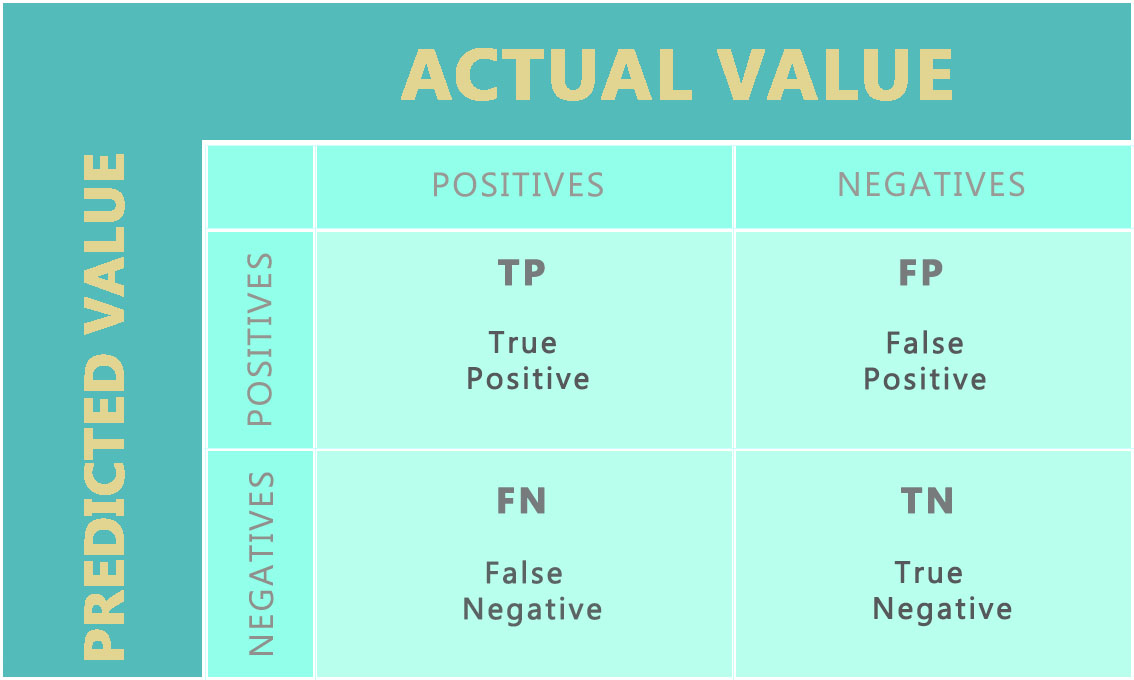
\includegraphics[scale=0.33]{Graphics/confusion-matrix.png}
    \caption{Confusion Matrix}
    \label{fig:confusion-matrix}
\end{figure}


Based on the above given categories, measurement metrics can be calculated. Some of them are given bellow:

\[ \textrm{False Positive Rate (FP-Rate)} = \frac{FP}{N}, \textrm{where } N \textrm{ stands for negatives.}  \]
\[ \textrm{True Positive Rate (TP-Rate)} = \frac{TP}{P}, \textrm{where } P \textrm{ stands for positives.}  \]


An discrete classifier have by definition a class label as output to a particular example (e.g \(Y\)/\(N\) for binary classification) \cite{Fawcett:2006:IRA:1159473.1159475}. The results can be easily represented on a basic ROC Graph (see figure\footnote{Figure is taken from the work of \cite{Fawcett:2006:IRA:1159473.1159475}}: \ref{fig:roc-graph}), where the \(x\) - axis is the FP-Rate and \(y\) is representing the TP-Rate. The best classifier/point on the graph is the one with the highest true positive and the lowest false negative rate (point \(D\) on our graph).
\begin{figure}[h!]
    \centering
    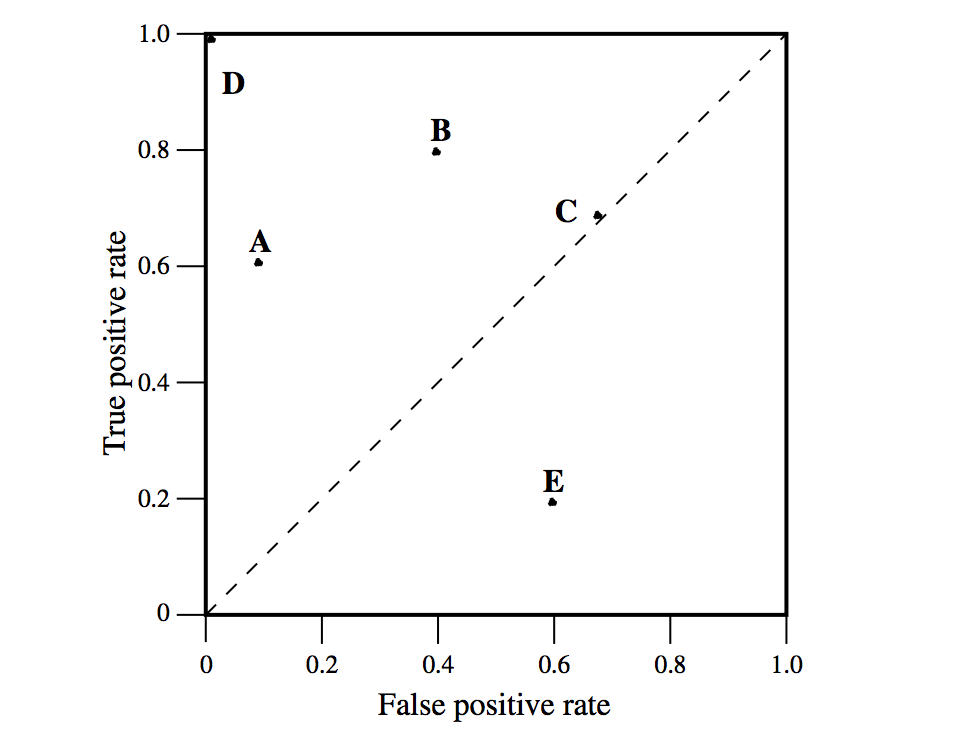
\includegraphics[scale=0.6]{Graphics/roc-graph.png}
    \caption{ROC-Graph for discrete classifier.}
    \label{fig:roc-graph}
\end{figure}

Moreover, a considerable case is the point \(C\) located on the diagonal dotted line. There the FP and TP rates are equivalent - ergo the classification probability is random.

Some classifier naturally yields a numeric value as a classification result of an example. These values are either strict probabilities or they can be uncalibrated scores, where a higher score indicate a higher probability. Although these values can be converted into binary labels by using a threshold e.g if the value is above the threshold then the label is \(Y\) else \(N\). So, each threshold would produce a different point into the ROC-Space, connecting the points together produce the ROC-Curve (see figure\footnote{Figure is taken from the work of \cite{Fawcett:2006:IRA:1159473.1159475}}:\ref{fig:roc-curve}). 

\begin{figure}[h!]
    \centering
    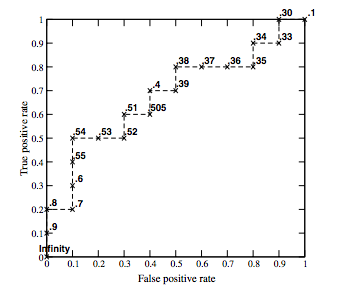
\includegraphics[scale=0.7]{Graphics/roc-curve.png}
    \caption{ROC-Curve for probabilistic classifier.}
    \label{fig:roc-curve}
\end{figure}

Another important property of ROC-Curve it is slightly sensitive to the distribution of particular classes in the data (e.g the proportions of FP-Rate <-> TP-Rate). This may an attractive feature if true negative is not much valuable to the problem, or negative examples are abundant but in the case of a fraud detection problem, where negative (fraud) examples are by definition rare, the ROC-Graph will not provide enough insides to measure classification right caused by skewed class distribution. Thus, additional metrics required.
Bellow, precision, and recall are given, both of them are sensitive to the class distribution due to the fact that the calculation is also related to the opposite classification category (TP-Rate is related to True Positives and the amount of positives where precision also include false negatives in the calculation):

\[ \textrm{Positive precision  (precision)} = \frac{TP}{TP+FN}  \]
\[ \textrm{Negative recall (recall)} = \frac{TN}{TN+FP}  \]

An example in figure\footnote{Figure is taken from the work of \cite{Fawcett:2006:IRA:1159473.1159475}} \ref{fig:roc-pr-curve} illustrate classification on two data sets differ by the amount of negatives. The curves on (a) and (c) (ROC-Curve) show up only a minimal change although a number of negatives is differed by 10 times, where the positive-recall graph on (b) and (d) differ substantially. 

\begin{figure}[h!]
    \centering
    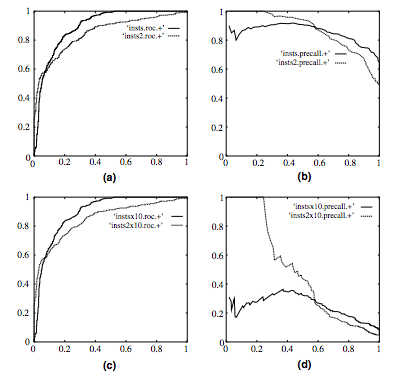
\includegraphics[scale=0.8]{Graphics/curves-vs-pr-analysis.png}
    \caption{ROC-Curve for probabilistic classifier.}
    \label{fig:roc-pr-curve}
\end{figure}

ROC analysis is a useful tool for measuring classifiers performance. With the concept of ROC graphs, a visualization technique is given to provide a richer
measure of classification performance than scalar measures
such as accuracy, error rate or error cost \cite{Fawcett:2006:IRA:1159473.1159475}. Moreover, precision - recall curves look promising to satisfy the needs of this thesis by the ability to evaluate classification algorithms used on a class-imbalanced data set.

